\documentclass{report}
\usepackage[T1]{fontenc}
\usepackage[utf8]{inputenc}
\usepackage[french]{babel}
\usepackage{color}
\usepackage{amsmath}
\usepackage{amssymb}
% Pour utiliser le signe €
\usepackage{eurosym}
% Pour pouvoir insérer des images
\usepackage{graphicx}
\graphicspath{images/}
% Pour pouvoir insérer des hyperliens
\usepackage[hyphens]{url}
\usepackage{hyperref}
% Suppression des marges supplémentaires sur les bords
\usepackage{fullpage}
% Forcer l'affichage des figures à un endroit précis
\usepackage{here}
% On ne veut pas afficher le mot 'Chapitre' avant chaque chapitre
\usepackage{titlesec}
\titleformat{\chapter}[hang]{\bf\huge}{\thechapter}{2pc}{}

% Pour les en-têtes et pieds de page
\usepackage{fancyhdr}
\renewcommand{\headrulewidth}{0pt}
\lhead{} 
\chead{} 
\rhead{} 
\renewcommand{\footrulewidth}{0pt}
\lfoot{Antoine Augusti} 
\cfoot{\thepage} 
\rfoot{statistics.teen-quotes.com} 
\pagestyle{fancy}

% Coloration syntaxique
\usepackage{listings}
\lstset{ 
	language=PHP,
	numbers=left,
	showstringspaces=false, 
	tabsize=4,
	breaklines=true,
	extendedchars=true,
	literate={é}{{\'e}}1 {à}{{\'a}}1 {è}{{\`e}}1 {ç}{{\c c}}1
}
%----------------------- %
% -- Cheat sheet -------- %

% Alignement
%\begin {flushleft}
%\begin {center}
%\begin {flushright}

% Listes
% \begin{itemize}
% \begin{description}
% \begin{enumerate}
% 	\item Numéro 1
% 	\item Numéro 2
% \end{enumerate}
% \\
% \newpage

% Mise en forme des caractères
% \normalfont{} ou \begin{rm}
% \textbf{} ou \begin{bf}
% \textit{} ou \begin{it}
% \textsc{} ou \begin{sc}
% Emphase (sémantique)
% \emph{}

% Citations et code brut
% \quote Pour une ligne isolée
% \quotation Pour un bloc
% \verb Pour du code
% \lstlisting Pour du code coloré

% URL
% \url{http://www.site.org/}
% ------------------------------------ %


% ------------------------------------ %
% -- METADONNÉES DU DOCUMENT --------- %
% Utilisées pour générer la page de garde
\title{
		Projet Final de M8\\
		Étude de Teen Quotes
}
\author{
	Antoine \textsc{Augusti}, 
}
\date{Juin 2013}

\begin{document}

	% Génération de la page de garde
	\maketitle

	% Génération de la table des matières
	\tableofcontents

	% ///////////////////////////////////////////////////////// %
	% /// Introduction //////////////////////////////////////// %
	\chapter{Introduction}
	% ------------------------------------------- %
	% -- Teen Quotes, qu'est-ce que c'est ? ----- %
	\section{Teen Quotes, qu'est-ce que c'est ?}
	Teen Quotes est une plateforme regroupant des citations décrivant le quotidien des adolescents. L'adolescence est une période difficile à gérer dans la vie et les adolescents ont souvent besoin d'échanger autour de sujets qui les préoccupent : leurs amis, l'amour, les études, leurs déceptions, leurs expériences. Teen Quotes répond à ce besoin en proposant à toute personne possédant un compte de pouvoir partager son impression en écrivant une courte citation. Cette citation sera ensuite acceptée (modifiée légèrement ou non) pour publication ou rejetée. Actuellement, cinq nouvelles citations sont publiées tous les jours à 0h (heure française) sur Teen Quotes.\\

	L'interface de Teen Quotes est proposée par défaut en anglais. L'interface est également disponible en français pour ceux qui le désirent et une version en français par défaut existe (elle se nomme Kotado). Toutefois, la version française de Teen Quotes ayant moins de succès que la version originale, j'ai choisi d'orienter mon projet de M8 vers cette version anglaise.\\

	Teen Quotes a été lancé en mai 2011, après quelques mois de développement que j'ai mené seul. Aujourd'hui Teen Quotes possède une version web pour les ordinateurs, une version optimisée pour les smartphones (depuis navigateur) ainsi qu'une application iPhone / iTouch que l'on peut télécharger depuis l'App Store d'Apple. Plus de 1,5 million de personnes ont visité Teen Quotes, depuis l'une des versions que nous proposons.\\

	Je me suis également associé depuis deux ans à une jeune femme philippine (parlant anglais) qui tient le compte Twitter de Teen Quotes (\href{http://twitter.com/ohteenquotes}{\textit{@ohteenquotes}}) comptant actuellement plus de 2 millions de followers. Nous essayons ensemble d'avoir une convergence vers tous les supports où Teen Quotes est présent (Twitter, Facebook, site web, site mobile, application iPhone / iTouch) pour agrandir notre masse d'utilisateurs.

	% ---------------------------------------------------- %
	% -- Et moi, je peux avoir accès à Teen Quotes ? ----- %
	\section{Et moi, je peux avoir accès à Teen Quotes ?}
	Bien évidemment ! Teen Quotes est ouvert à tout le monde et mon but est que le plus de monde possible rejoigne l'aventure. Teen Quotes peut être consulté grâce aux moyens suivants :
	\vspace{10px}
	\begin{itemize}
		\item Site web : \url{http://teen-quotes.com}
		\item Site mobile \footnote{Lien à visiter depuis un smartphone ou une tablette. La redirection vers la version mobile est automatique quand on tente de visiter le site classique depuis un smartphone ou une tablette.} : \url{http://m.teen-quotes.com}
		\item Application iPhone / iTouch \footnote{Lien à visiter depuis un iPhone ou un iTouch pour lancer le téléchargement de l'application !} : \url{http://teen-quotes.com/apps}
	\end{itemize}

	% ---------------------------------------------------- %
	% -- Des données oui, mais des données à jour -------- %
	\section{Des données oui, mais des données à jour}
	Teen Quotes enregistre plus de \textbf{4 000 visites par jour}. Les bases de données de Teen Quotes enregistrent environ \textbf{30 000 requêtes par heure}. Avec un tel volume de données, difficile de se contenter d'une étude statistique figée, obslète une semaine plus tard car les données ne sont plus du tout les mêmes. Teen Quotes est vivant, évolue en permanence : l'étude statistique de Teen Quotes doit s'adapter en conséquence.\\

	En réponse à ce défi, j'ai décidé d'orienter mon projet de M8 vers une étude statistique évolutive, qui se renouvelle en permanence et qui a pour ambition de donner des informations correctes et précises en quasi temps réel. Pour répondre à ce besoin, quoi de mieux que de proposer une étude en ligne ? Facile à consulter : il suffit d'un navigateur web.

	% Comment ça fonctionne ?
	\subsection{Comment ça fonctionne ?}
	L'idée était donc de créer une partie du site de Teen Quotes dédiée aux statistiques : affichage de graphiques et informations sur les données. Les données sont recalculées 3 fois par heure (soit toutes les 20 minutes si vous suivez !). La réflexion suivie pour arriver à ceci a donc été la suivante :
	\vspace{10px}
	\begin{enumerate}
		\item Quelles sont les données que je veux afficher ?
		\item Comment est-ce que je peux récupérer ces données ? Sont-elles enregistrées dans mes bases de données ou sur un service externe (Google Analytics \footnote{Google Analytics fournit une analyse d'audience pour le site web classique et le site web mobile.}, Flurry \footnote{Flurry fournit des données sur les utilisateurs de l'application iPhone / iTouch.}) ?
		\item Comment faut-il rassembler les données ? Comment donner du sens aux données brutes ? Comment les formater ?
		\item Comment proposer un affichage agréable et lisible pour donner sens aux données récupérées ?
		\item Comment automatiser tout ce processus pour pouvoir effectuer une mise à jour des informations toutes les 20 minutes ?
	\end{enumerate}
	\vspace{10px}
	Le résultat final est visible à l'adresse \url{http://statistics.teen-quotes.com} et est disponible en anglais (dans un souci d'intérêt pour le public visé par Teen Quotes !) et en français. Je vous invite fortement à vous rendre à cette adresse, la suite du rapport expliquant en détail chaque graphique affiché sur cette page.\\

	Des précisions techniques seront apportées au fur et à mesure du rapport pour vous faire une idée de comment est réalisée cette page.

	% ///////////////////////////// %
	% /// Qui vient chez nous ? /// %
	\chapter{Qui vient chez nous ?}
	Quand nous avons décidé de lancer Teen Quotes, nous ne savions qu'une chose : il fallait que le site soit en anglais pour toucher le plus de monde possible à travers le globe. Partout dans le monde où il y avait un accès à Internet et où les gens parlaient anglais, nous devions pouvoir être accessibles.\\

	Nous n'avions pas une population cible précise et pas de préférence particulière pour un ou des pays. La communication n'a jamais été orientée vers une quelconque culture ou un quelconque continent. Les statistiques obtenues sont donc une régulation naturelle des flux vers Teen Quotes.

	% ------------------------------------------ %
	% -- Où habites-tu petit visiteur ? -------- %
	\section{Où habites-tu petit visiteur ?}
	La première chose à déterminer est la localisation géographique de connexion des visiteurs pour accéder à Teen Quotes. Ceci nous permet d'avoir en notre possession plusieurs informations importantes :
	\vspace{10px}
	\begin{itemize}
		\item Une connaissance de notre audience dans l'éventualité de s'orienter plus vers un pays ou un continent pour des opérations futures.
		\item Un besoin d'optimisation technique vers les pays de grande audience : nos serveurs sont en France mais très peu de visiteurs visitent Teen Quotes depuis la France.
	\end{itemize}
	\vspace{10px}
	Les données de localisation des visites sont données par Google Analytics pour le site web et le site pour mobiles. Les données de localisation pour l'application iPhone / iTouch sont fournies par Flurry. Flurry se contente de donner des informations au niveau des continents alors que Google Analytics est capable de déterminer la localisation au niveau des villes de taille moyenne (Rouen par exemple). Dans un souci de respect de la vie privée des utilisateurs, on se limite à une localisation au niveau de la ville moyenne la plus proche de son lieu de connexion.\\

	On s'intéresse à la totalité des visites de Teen Quotes depuis la création en mai 2011 jusqu'en juin 2013 : on compte donc des personnes en double, forcément. Toutefois il est impossible de faire autrement : les visiteurs peuvent se déplacer géographiquement, changer d'adresse IP... La seule solution pour éviter les doublons serait de ne s'intéresser qu'aux visites de personnes authentifiées sur Teen Quotes, ce qui nous priverait d'une bonne partie des données.\\

	Comme on souhaite s'intéresser aux visites par pays, on ne retient que les données de localisation du site web et du site optimisé pour mobiles en laissant de côté les données de localisation de l'application iPhone / iTouch qui a été lancée en novembre 2012.
	\begin{figure}[H]
		\center
		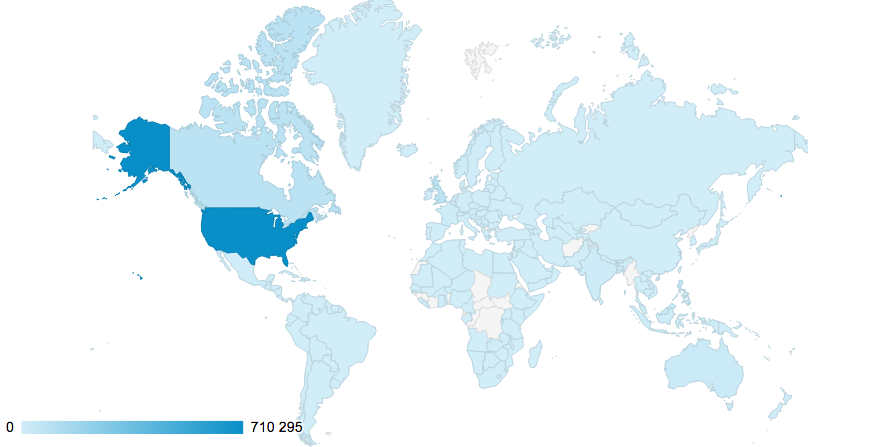
\includegraphics[width=400px]{images/visitesMondialesCarte.png}
		\caption{Visites depuis la création de Teen Quotes représentées sur une carte mondiale.}
	\end{figure}
	On a appliqué un dégradé de bleu pour symboliser le nombre de visites : le bleu foncé représentant le pays avec le plus de visiteurs.\\
	De cette carte on peut tirer l'analyse suivante :
	\vspace{10px}
	\begin{itemize}
		\item Quasiment tous les pays du monde sont coloriés en bleu : c'est-à-dire qu'il y a eu au moins une visite depuis 211 pays ou États\footnote{On obtient ce chiffre en regardant la liste des pays qui ont enregistré au moins une visite, et non en les comptant sur la carte !} dans le monde. Les pays grisés sont majoritairement situés en Afrique : l'absence de visites depuis ces pays peut s'expliquer par le faible taux d'accès à Internet pour les particuliers.
		\item Les visites depuis les États-Unis ont l'air très majoritaires, à tel point qu'il est difficile de voir une différence pour les autres visites tant les écarts sont grands entre le pays le plus visité et les autres.
	\end{itemize}
	\vspace{10px}
	Pour mieux visualiser le poids de chaque poids, représentons les visites sur un diagramme circulaire.
	\begin{figure}[H]
		\center
		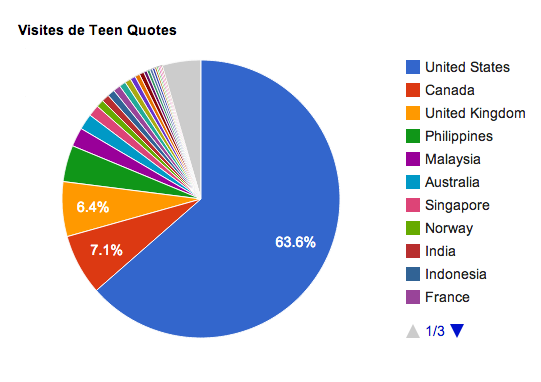
\includegraphics[width=250px]{images/visitesMondialesCamembert.png}
		\caption{Visites depuis la création de Teen Quotes représentées sur un diagramme circulaire.}
	\end{figure}
% Fin du do\cument
\end{document}